In Figure~\ref{fig:architecture} is depicted the architecture of KDM-RE which is split in three layers. As shown in this figure, the first layer of our \textit{plug-in} is the Core Framework. This layer represents that  we devised the  \textit{plug-in} on the top of the Eclipse Platform. In this layer it is also possible to see that we  used both Java and Groovy as programming language. Moreover, this layer contains Eclipse Plugins on which our tool is based on, such as MoDisco and EMF. We used MoDisco\footnote{http://www.eclipse.org/MoDisco/} that is an extensible framework to develop model-driven tools to support use-cases of existing software modernization and provides an Application Programming Interface - (API) to easily access the KDM model. Also, Eclipse Modeling Framewokr (EMF)\footnote{http://www.eclipse.org/modeling/emf/} was used to load and navigate KDM models that were generated with MoDisco. 

The second layer, the Tool Core, is where all refactorings provided by our \textit{plug-in} were implemented. KDM-RE works intensively with KDM models, which are XML files. Therefore, we use Groovy to handle those types of files because of the simplicity of its syntax and fully integrated with Java. KDM-RE also provides a way to create multiple versions of the KDM file to allow the engineer  to assess different refactorings in the same system. In order to optimizes memory usage of multiple versions for large models and enabling to work interactively on multiple models our \textit{plug-in} persists these models in a MongoDB. We chose MongoDB since it provides a high performance. After the engineer to choose a version refactored a forward engineering is carried out and the source code of the modernized target system is generated again. Finally, the top layer is the Graphical User Interface (GUI) that consists of a set of SWT windows with several options to perform the refactorings based on the KDM model.


\begin{figure}[!ht]
\centering
  % Requires \usepackage{graphicx}
  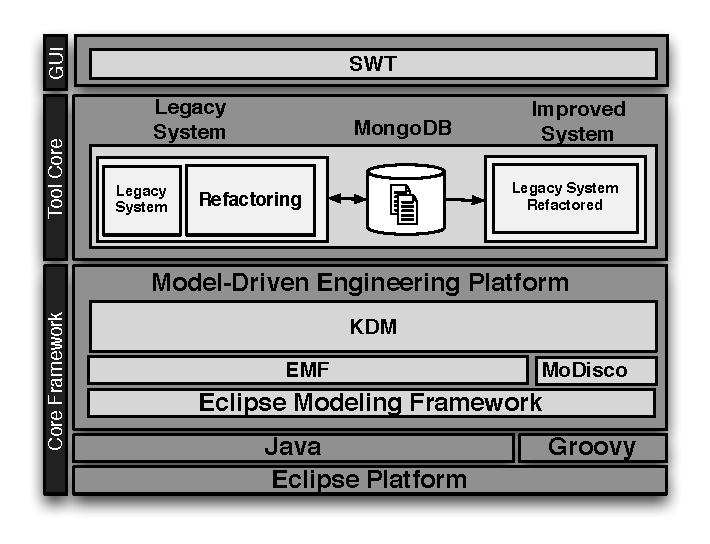
\includegraphics[scale=0.8]{figure/Arquitetura}
\caption{Architecture of KDM-RE}
\label{fig:architecture}
\end{figure}  